\documentclass[a4paper,10pt]{article}

%A Few Useful Packages
\usepackage{marvosym}
\usepackage{fontspec} 					%for loading fonts
\usepackage{xunicode,xltxtra,url,parskip} 	%other packages for formatting
\RequirePackage{color,graphicx}
\usepackage[usenames,dvipsnames]{xcolor}
%\usepackage[big]{layaureo} 				%better formatting of the A4 page
% an alternative to Layaureo can be ** \usepackage{fullpage} **
\usepackage[empty]{fullpage}
\usepackage{supertabular} 				%for Grades
\usepackage{titlesec}					%custom \section
\usepackage{tabu}
\usepackage{multirow}
\usepackage{hyperref}


%Setup hyperref package, and colours for links
\usepackage{hyperref}
\definecolor{linkcolour}{rgb}{0,0.2,0.6}
\hypersetup{colorlinks,breaklinks,urlcolor=linkcolour, linkcolor=linkcolour}

%FONTS
\defaultfontfeatures{Mapping=tex-text}
%\setmainfont[SmallCapsFont = Fontin SmallCaps]{Fontin}
%%% modified for Karol Kozioł for ShareLaTeX use
\setmainfont[
SmallCapsFont = Fontin-SmallCaps.otf,
BoldFont = Fontin-Bold.otf,
ItalicFont = Fontin-Italic.otf
]
{Fontin.otf}
%%%

%CV Sections inspired by: 
%http://stefano.italians.nl/archives/26
\titleformat{\section}{\Large\scshape\raggedright}{}{0em}{}[\titlerule]
\titlespacing{\section}{0pt}{2pt}{2pt}
%Tweak a bit the top margin
   \addtolength{\voffset}{-0.7cm}
%\vsize=15cm
%\setlength{\footskip}{.96cm}
%\def\makefootline{\baselineskip24pt\lineskiplimit0pt\line{\the\footline}}
%\vsize 180mm
%\addtolength{\vsize}{-50cm}
%Italian hyphenation for the word: ''corporations''
\hyphenation{im-pre-se}

%-------------WATERMARK TEST [**not part of a CV**]---------------
\usepackage[absolute]{textpos}

\setlength{\TPHorizModule}{30mm}
\setlength{\TPVertModule}{\TPHorizModule}
\textblockorigin{2mm}{0.80\paperheight}
\setlength{\parindent}{0pt}
%\setlength{\topsep}{5pt}%

%--------------------BEGIN DOCUMENT----------------------
\begin{document}

\pagestyle{empty} % non-numbered pages

\font\fb=''[cmr10]'' %for use with \LaTeX command

%--------------------TITLE-------------



  \begin{tabular}{ p{11.5cm}r }
   & \multirow{2}{*}{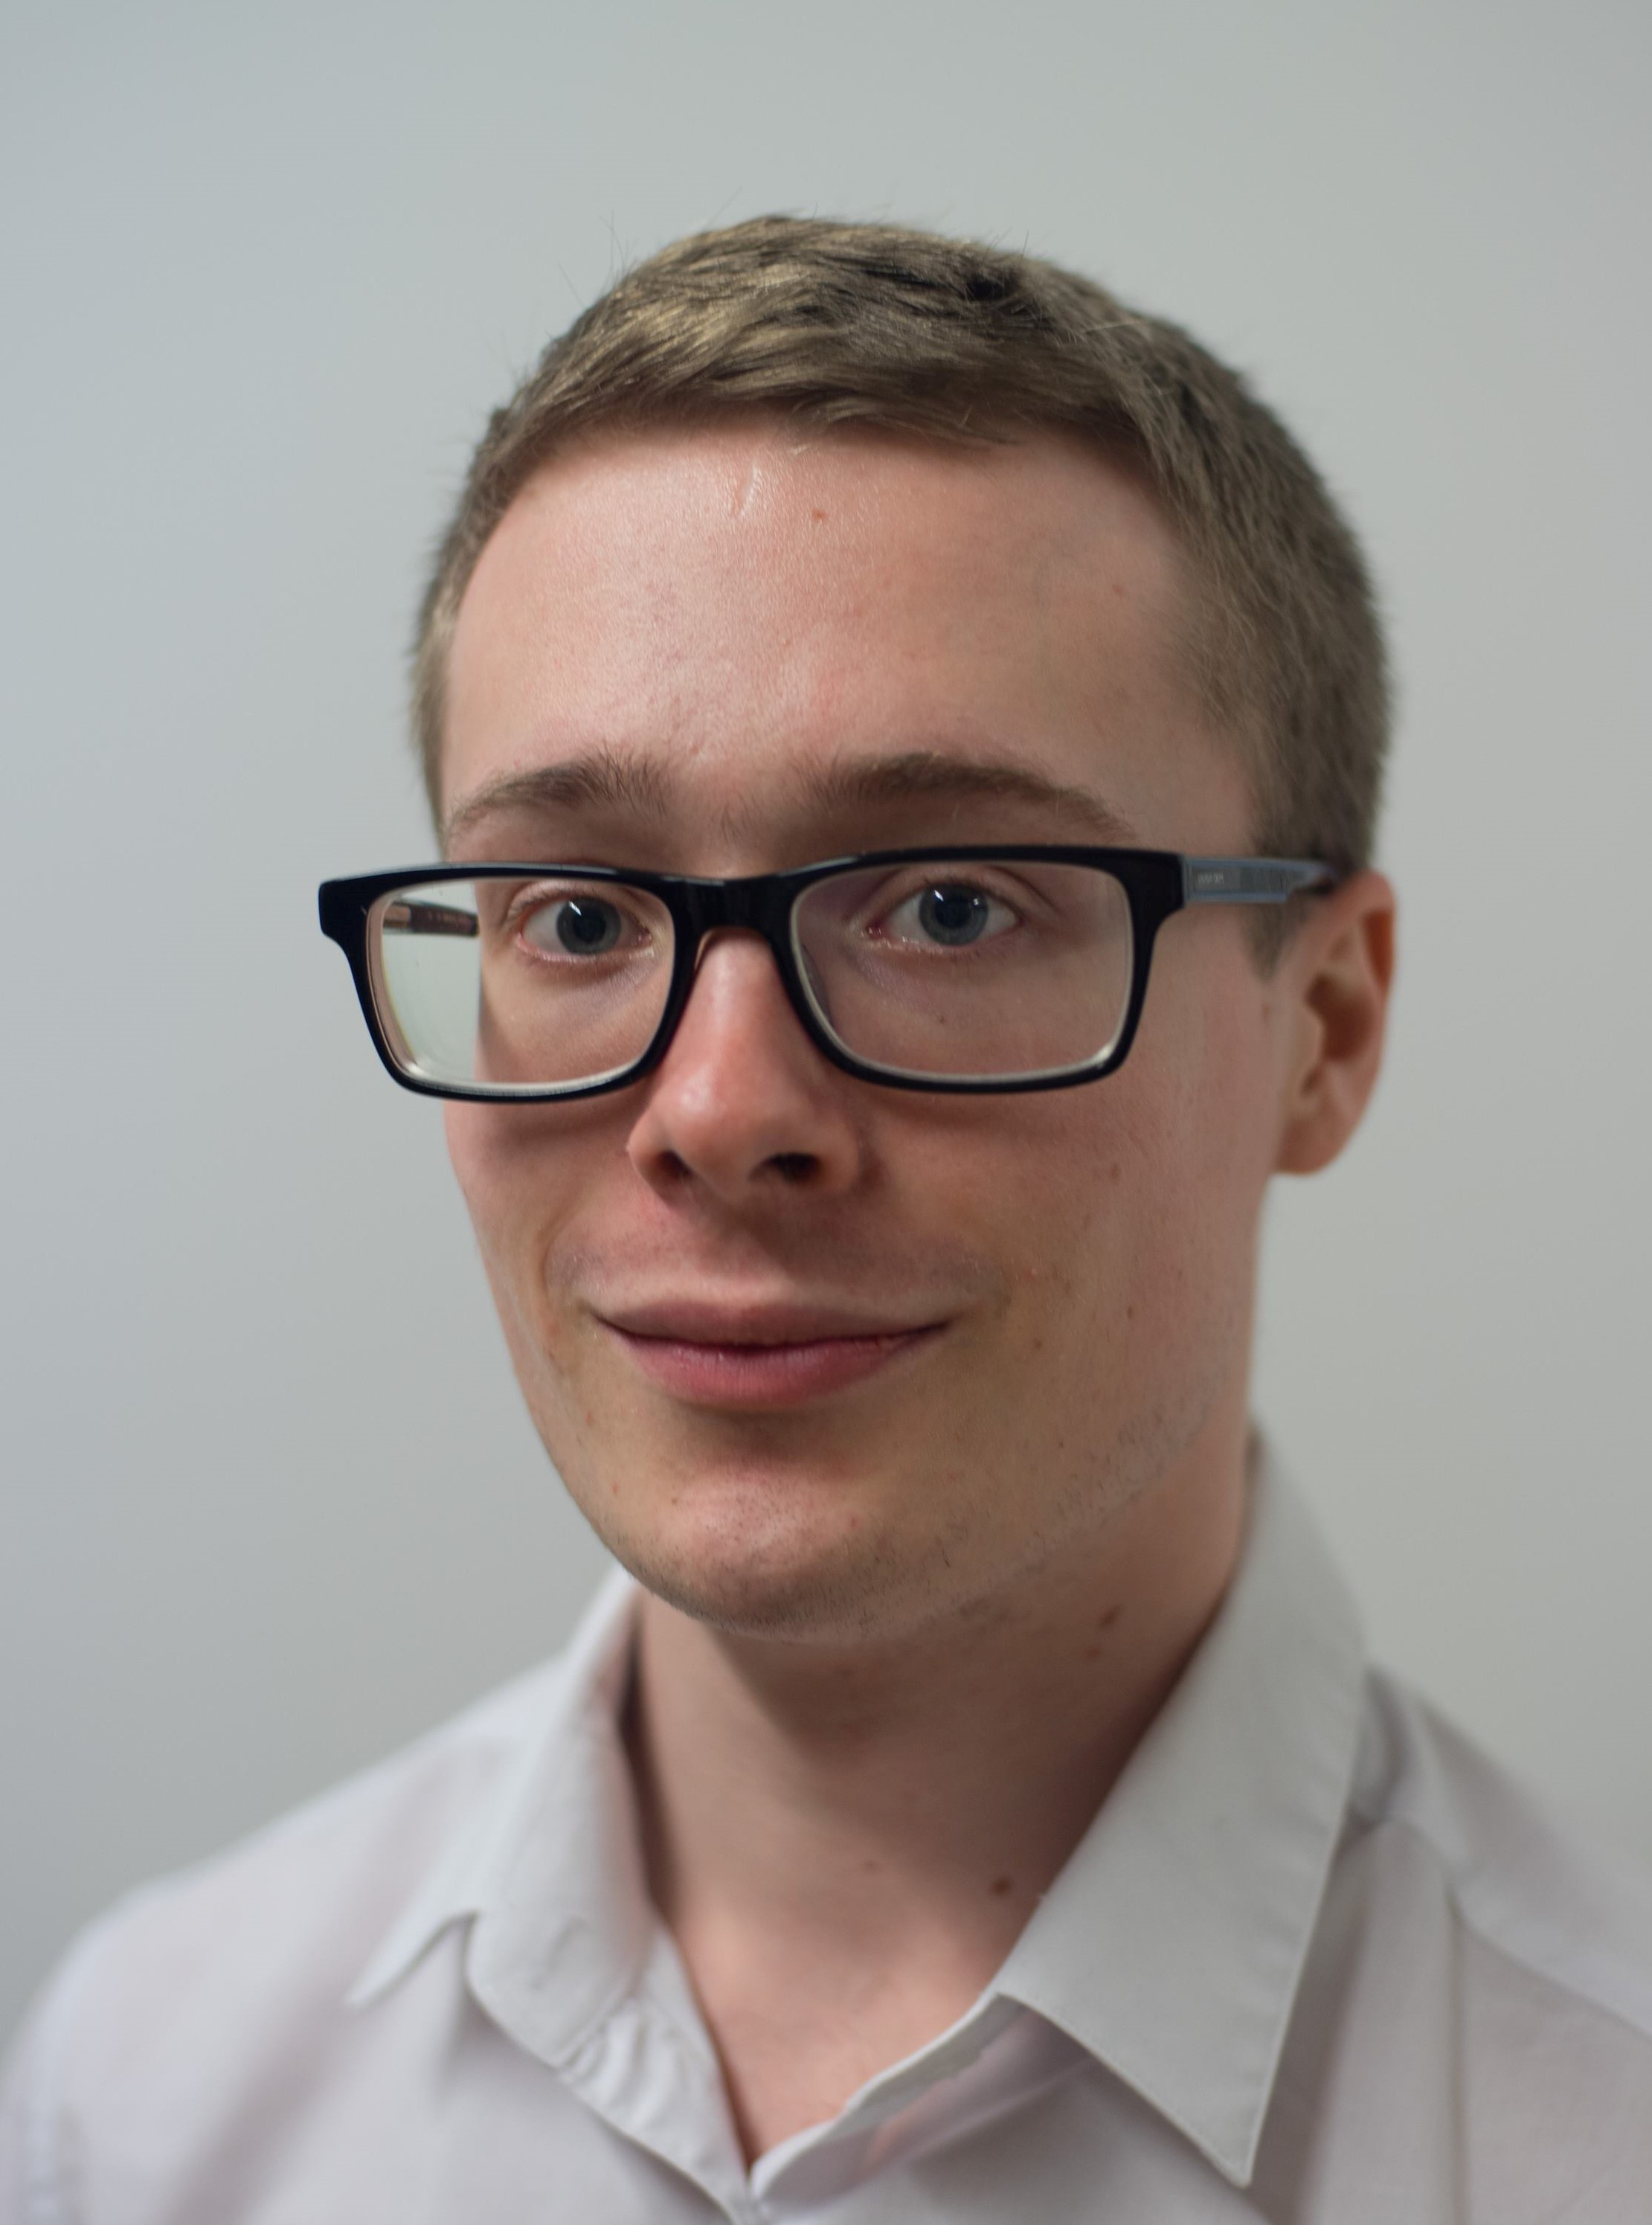
\includegraphics[width=1.3in]{pic}}\\
   \\
   \scshape{\Huge{Charles Nourry}} & \\
   \\
   \textsc{Date de naissance :} 12/12/1996 &\\
    \textsc{Adresse :} 1 rue de la ferme &\\
    \textsc{Ville :} 78150 - Le Chesnay&\\
    \textsc{Pays :} France&\\
    \textsc{Téléphone :} 06 21 09 85 62&\\
    \textsc{e-mail :} \href{mailto:nourry\_charles@outlook.fr}{nourry\_charles@outlook.fr}& %\multirow{5}{2in}{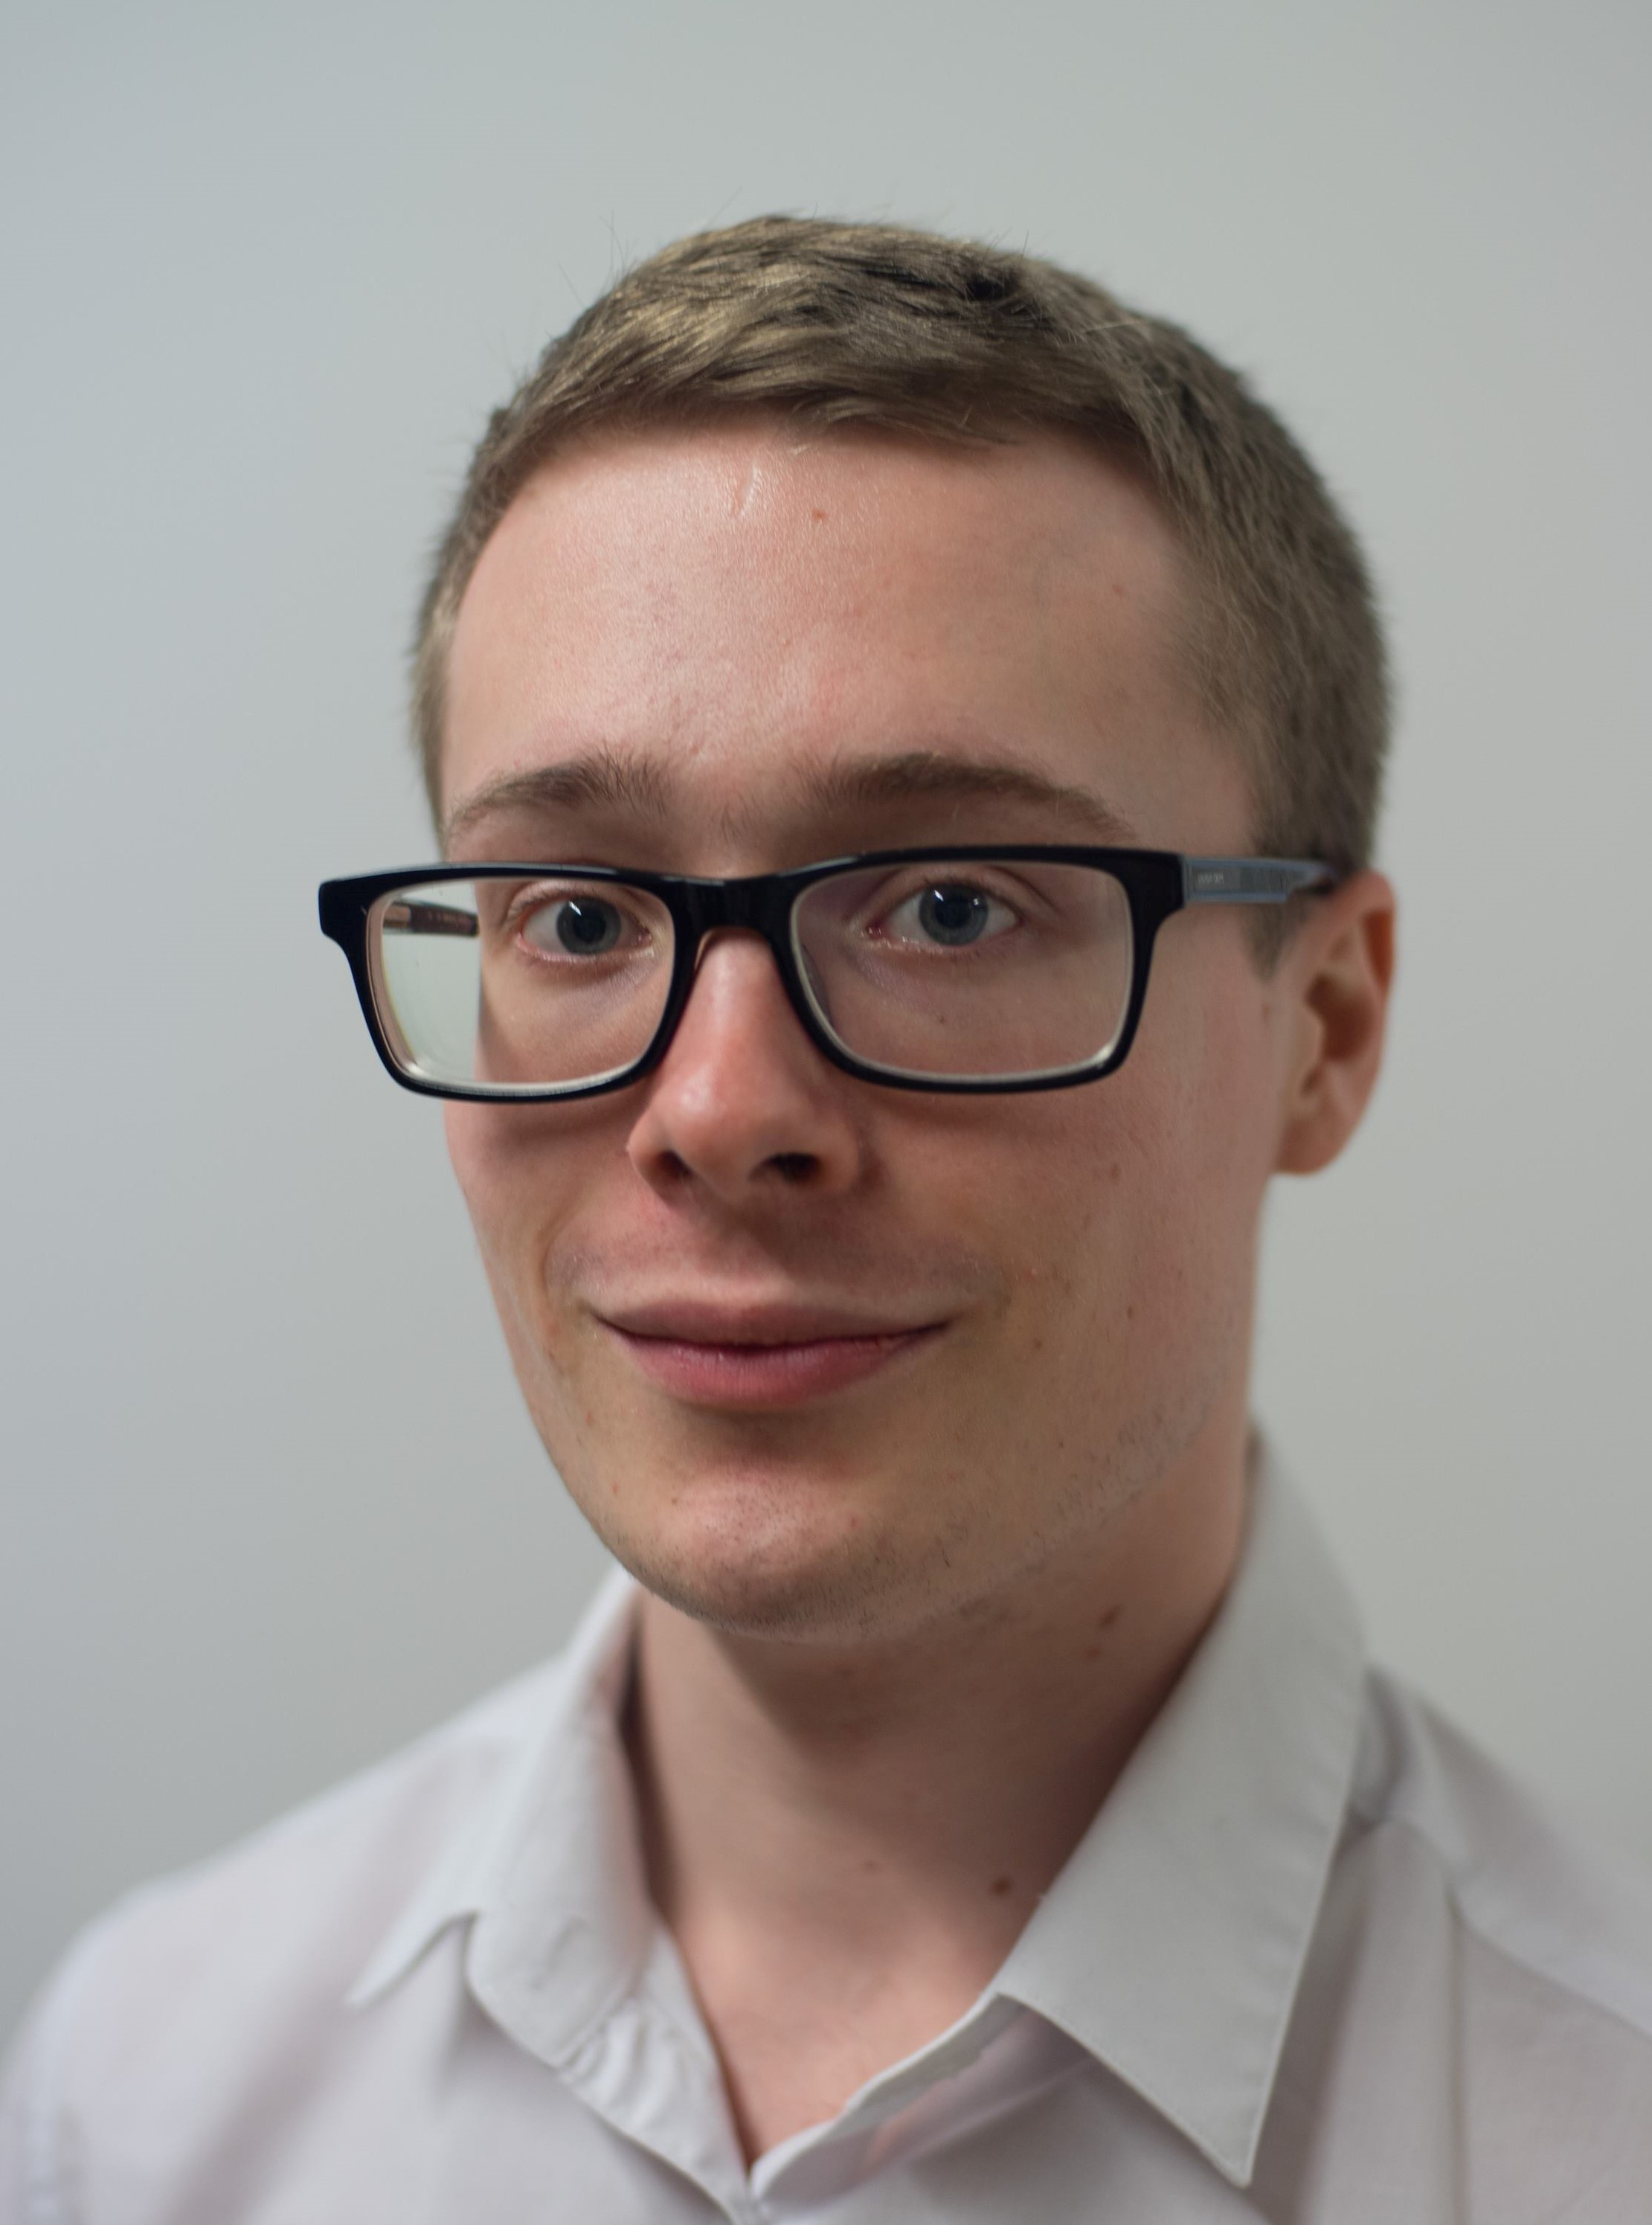
\includegraphics[width=1.5in]{pic}}
  \end{tabular}
  
  %TITRE
  \vspace{0.1in}
  %\centering{
  %\Large{Candidature à l'offre de stage : Optimisation de l’insertion de contre mesure pour la sécurité des Circuits Intégrés}
%}

%--------------------SECTIONS-----------------------------------
%Section: Personal Data
%\section{Personal Data}

%\begin{tabular}{ll}
 %   \textsc{Age:} & 20 \\
  %  \textsc{Address:}   & 1 rue de la ferme \\
%    \textsc{Ville:} 	& 78150 - Le Chesnay\\
 %   \textsc{Phone:}     & 06 21 09 85 62\\
  %  \textsc{email:}     & $\href{mailto:nourry_charles@outlook.fr}{nourry_charles@outlook.fr}$
%\end{tabular}

%Section: Work Experience at the top
\section{Formation}
\begin{tabular}{p{0.06cm} c p{0.04cm}|p{13cm}}
 & \textsc{oct. 2019-} & & Doctorat en informatique - "Conception multi-objectifs de réseaux et polyhèdres"\\
 & & & Sujet : au LAMSADE \emph{}\\
 & & & \emph{\small{Encadré par Ali Ridha Mahjoub et Hassène Aissi}}\\\multicolumn{2}{c}{}\\
 & \textsc{2018-2019} & & Master 2 Modélisation, Optimisation, Décision et Organisation (Major M1 \& M2)\\&&&\emph{\small{Cohabilité par l'Université Paris-Dauphine et Mines ParisTech}}\\\multicolumn{2}{c}{} \\
 %& \textsc{2017-2018} & & Master 1 Parcours Informatique pour la Décision (Major)\\&&&\emph{\small{Université Paris-Dauphine}}\\\multicolumn{2}{c}{} \\
 & \textsc{2016-2017} & & Licence Informatique des organisations - MIAGE et Décision (Major)\\&&&\emph{\small{Université Paris-Dauphine}}\\\multicolumn{2}{c}{} \\
 & \textsc{2014-2016} & & Diplôme d'Etablissement Mathématiques, Informatique et applications à l'Economie et à l'Entreprise (L1 \& L2) \\&&&\emph{\small{Université Paris-Dauphine}}\\\multicolumn{2}{c}{} \\
 &\textsc{2014} & & Baccalauréat Scientifique option Mathématiques \\&&&\emph{\small{Lycée Blanche de Castille, Le Chesnay}}\\
\end{tabular}
\titlespacing{\section}{0pt}{2pt}{2pt}
\section{Expériences personnelles}
\begin{tabular}{c|l}	
\textsc{octobre} 2019 & Enseignement Université Paris-Dauphine \\ 
 \textsc{mai} 2024 & Programmation Linéaire, Java, Optimisation combinatoire, Algoritmique et programmation,\\
  & Théorie des graphes, Aide à la décision, Python, Linux. \\
 & \emph{de fibres optiques"}\small{ - Modélisation et optimisation à l'aide d'approches exactes en PLNE}\\\multicolumn{2}{c}{} \\
 \textsc{avril} 2019 & Stage de fin de Master au sein d’\textsc{Orange Labs Networks} \\ 
 \textsc{septembre} 2019 & \emph{"Chargé de conception de modèles et algorithmes d'optimisation pour réseaux}\\
 & \emph{de fibres optiques"}\small{ - Modélisation et optimisation à l'aide d'approches exactes en PLNE}\\\multicolumn{2}{c}{} \\
 &\small{Finaliste Prix du mémoire de Master RO/AD de la ROADEF 2019}
 \textsc{mai} 2018 & Stage de recherche au \textsc{LAMSADE} (Laboratoire d'Analyse et de Modélisation de\\  \textsc{août} 2018 & Systèmes pour l'Aide à la Décision) - Université Paris-Dauphine\\
  & \emph{"Analyse de débats en ligne"}\small{ - Modélisations de débats à l'aide de la théorie de l'argumentation}\\\multicolumn{2}{c}{} \\
 \textsc{mai} 2017 & Stage de Licence au \textsc{Crédit Industriel et Commercial}\\
 \textsc{août} 2017 & \emph{"Mise en place d'outils informatiques"}\small{ - Gestion de bases de données et élaborations} \\ &  \small{d'applications}\\\multicolumn{2}{c}{}
 \end{tabular}

\section{Compétences}

\begin{tabular}{l p{15cm}}	
\textsc{Domaine :}    &   Optimisation Combinatoire, Programmation Mathématique, Modélisation, Aide à la décision\\&\\
\textsc{Développement :} & CPLEX, Programmation orientée objet, Java, Julia, C, Python, R, Matlab, \LaTeX, VBA\\&\\
\textsc{Logiciels/OS :}&  Microsoft Windows, Linux, CPLEX  Studio, GitHub, Jupyter Notebook, RStudio, Eclipse, \\
     &                    JetBrains (\emph{IntelliJ, CLion, PyCharm,...}), MySQL, Word, Excel, PowerPoint, Access
\end{tabular}


%Section: Languages
\section{Langues}
\begin{flushleft}
\begin{tabular}{p{0.05cm}ll}
&\textsc{Français :}&Langue maternelle\\
&\textsc{Anglais :}&Courant (TOEIC 2018: 820/990)\\
&\textsc{Espagnol :}&Occasionnel
\end{tabular}
\end{flushleft}

\end{document}
%\section{Centres d'intérêt}
%\begin{flushleft}
%Piano, Cinéma, Athlétisme
%\end{flushleft}
%\XeTeXpdffile ''GMAT.pdf'' page 1 scaled 800
